%29/11 - Lucía Sánchez
\part{Genome/Phenome Analysis}
\chapter{Genome-Wide Association Studies (GWAS)}
\section{Introducción a GWAS y características}
Los \textbf{estudios de asociación a nivel del genoma} (GWAS, por sus siglas en inglés) son un enfoque utilizado para identificar variantes genéticas asociadas a rasgos o enfermedades específicas en una población. Estos estudios analizan la asociación entre \textbf{variantes genéticas comunes} y fenotipos mediante el genotipado de grandes cantidades de SNPs (Single-Nucleotide Polymorphisms) en múltiples individuos.

El gráfico ilustra la relación entre \textbf{frecuencia alélica} y \textbf{penetrancia}. La penetrancia mide el porcentaje de individuos portadores de una variante genética que desarrollan un fenotipo o enfermedad. Por otro lado, la frecuencia alélica indica la proporción en la población de un alelo determinado que causa un fenotipo.
\begin{itemize}
\item \textbf{Enfermedades mendelianas:} tienen alta penetrancia (con una mutación se desarrolla la enfermedad) pero baja frecuencia alélica. Un ejemplo es la talasemia, una enfermedad autosómica recesiva que afecta la síntesis de las cadenas alfa y beta de la hemoglobina, provocando anemia severa.
\item \textbf{Enfermedades complejas:} tienen baja penetrancia pero alta frecuencia alélica. GWAS se enfoca en estas variantes comunes que influyen parcialmente en el riesgo de enfermedades complejas como las enfermedades cardiovasculares, que involucran factores genéticos y ambientales.
\end{itemize}

\begin{figure}[htbp]
\centering
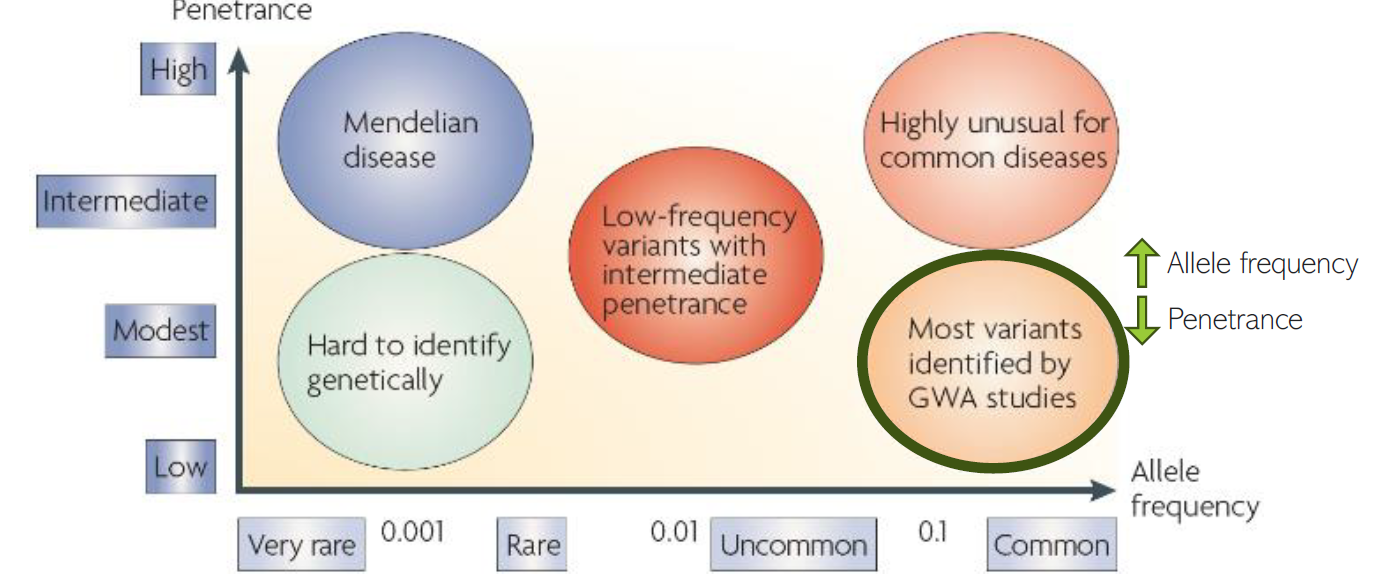
\includegraphics[width = \textwidth]{figs/gwas.png}
\end{figure}

Las variantes estudiadas en GWAS son:
\begin{itemize}
\item Single-Nucleotide Variant (SNV): Cambios de una sola base en el ADN causados por errores durante la meiosis o daño en el ADN de las células germinales.
\item Single-Nucleotide Polymorphism (SNP): SNVs presentes en al menos un 1\% de la población.
\end{itemize}

GWAS analiza grandes cantidades de SNPs (entre 500,000 y 1,000,000 por muestra). Esto es posible gracias a plataformas tecnológicas como Illumina y Affymetrix.

Las herramientas utilizadas en GWAS son:
\begin{itemize}
\item PLINK: Software especializado en la manipulación, resumen y limpieza de datos genéticos.
\item R: Utilizado para análisis estadístico y visualización.
\item Bases de datos:
\begin{itemize}
\item dbSNP: Para obtener información sobre variantes conocidas.
\item GWAS Catalog: Repositorio de estudios GWAS publicados.
\end{itemize}
\end{itemize}

\section{Realizar un GWAS}
El primer paso es \textbf{seleccionar una población de estudio}. Esto depende de la pregunta experimental y hay que tener un tamaño muestral suficiente para asegurar potencia estadística. Si el estudio es dicotómico, habría que tener casos y controles para ver la asociación entre presencia y ausencia. Si por el contrario el estudio es cuantitativo, hay que tener medidas cuantitativas. 

A las personas se las \textbf{genotipa} mediante Whole-genome Sequencing (WGS), whole-exome sequencing (WES) o microarrays (análisis de SNPs concretos para analizar variantes preseleccionadas). 

Una vez secuenciados los datos, hay que \textbf{procesarlos}. En algunos casos hay que anonimizar los datos, ver si hay relaciones familiares entre muestras, sexo, información fenotípica, etc. También es necesario realizar control de calidad. La imputación permite predecir variantes no genotipadas mediante patrones de asociación conocidos. Por último, se realiza un \textbf{test de asociación} para analizar la relación entre variantes genéticas y el fenotipo.

\subsection{Control de calidad}
\subsubsection{Missingness}
En el control de calidad, se mira el missingness o la ausencia tanto por SNP como por individuo. Se eliminan los SNPs o individuos con altos porcentajes de datos ausentes. Los valores recomendados son tener al menos un 95\% de información por muestra y un 95-99\% de información por SNP (call rate).

\begin{figure}[htbp]
\centering
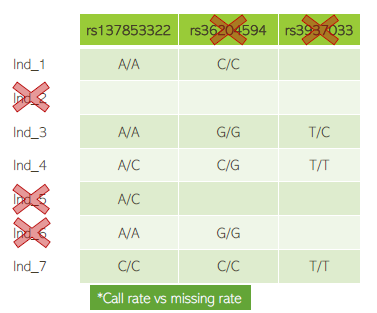
\includegraphics[width = 0.8\textwidth]{figs/missingness.png}
\end{figure}

\subsubsection{Discrepancia por sexo}
Se verifica la concordancia entre el sexo genotípico (tasa de homocigosis en el cromosoma X) y el sexo declarado.

%Para estudiar la discrepancia por sexo, se mira la diferencia entre el sexo asignado y el determinado basado en la información genotípica. Se determina mediante la computación de la tasa de homocigosis de los SNP del cromosoma X.

\subsubsection{Minor Allele Frequency (MAF)}
El Minor Allele Frequency (MAF) se define como la frecuencia del alelo menos frecuente en cada locus. Los GWAS se centran en variantes comunes asociadas a enfermedades en la población. Las variantes raras tienen baja potencia estadística.
Las variantes con un MAF muy bajo también se ven afectadas más fácilmente por errores de genotipado. Se utilizan los siguientes límites: 1-5\% para GWAS de unos cientos o mil individuos y más bajo (0,1\%) para tamaños muestrales más grandes, como UK Biobank.

\subsubsection{Hardy-Weinberg Equilibrium (HWE)}
El equilibrio de Hardy-Weinberg o ley de Hardy-Weinberg establece que en un apareamiento aleatorio tanto las frecuencias alélicas como genotípicas de una población permanecen invariables. Para que este equilibrio se dé, se deben cumplir los siguientes supuestos: apareamiento aleatorio, alelos femeninos y masculinos independientes, frecuencias alélicas idénticas entre machos y hembras, tamaño poblacional grande (infinito), no hay efecto de migración, mutación o selección natural. Para calcular las frecuencias genotípicas, se utiliza la siguiente fórmula:
$$P(G_i) = \sum_{j=1}^6 P(G_i|MT_j) \cdot P(MT_j)$$

\begin{figure}[htbp]
\centering
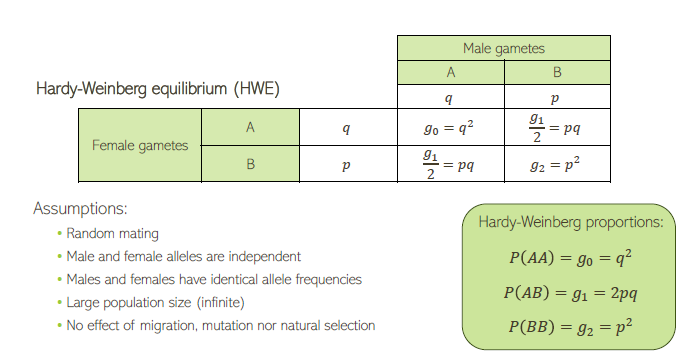
\includegraphics[width = \textwidth]{figs/hwe.png}
\end{figure}

Para asimilar esto, vamos a realizar un ejercicio en el que calculamos el equilibrio Hardy-Weinberg:
\begin{table}[h!]
\centering
\begin{tabular}{|l|c|ccc|}
\hline
\textbf{Mating types} & \textbf{Frequency} & \multicolumn{3}{c|}{\textbf{Frequency of zygotes}} \\ 
\cline{3-5}
                      &                    & \textbf{AA} & \textbf{AB} & \textbf{BB} \\ \hline
MT1: AA x AA          & $g_0g_0 = g_0^2$   & 1           & -           & -           \\
MT2: AA x AB          & $g_0g_1+g_1g_0 = 2g_0g_1$ & 0.5         & 0.5         & -           \\
MT3: AA x BB          & $g_0g_2 + g_2g_0= 2g_0g_2$ & -           & 1           & -           \\
MT4: AB x AB          & $g_1g_1 = g_1^2$   & 0.25        & 0.5         & 0.25        \\
MT5: AB x BB          & $g_1g_2+g_2g_1 = 2g_1g_2$ & -           & 0.5         & 0.5         \\
MT6: BB x BB          & $g_2g_2 = g_2^2$   & -           & -           & 1           \\ \hline
\end{tabular}
\caption{Tabla de frecuencias de tipos de apareamiento y cigotos.}
\label{tab:zygotes}
\end{table}

En base a los resultados de la tabla \ref{tab:zygotes}, las frecuencias genotípicas son:
$$q^2 = P(AA) = 1 \cdot g_0^2 + \frac{2g_0g_1}{2} + \frac{g_1^2}{4} = g_0^2 + g_0g_1 + \frac{g_1^2}{4} = (g_0 + \frac{g_1}{2})^2$$
$$p^2 = P(BB) = \frac{g_1^2}{4} + \frac{2g_1g_2}{2} + g_2^2 = \frac{g_1^2}{4} + g_1g_2 + g_2^2 = (g_2 + \frac{g_1}{2})^2$$
$$2pq = P(AB) = \frac{2g_0g_1}{2} + 1 \cdot 2g_0g_2 + \frac{g_1^2}{2} + \frac{2g_1g_2}{2} = g_0g_1 + 2g_0g_2 + \frac{g_1^2}{2} + g_1g_2 = 2(g_2 + \frac{g_1}{2})(g_0 + \frac{g_1}{2})$$

Para testar las proporciones HWE, se utiliza el test del chi cuadrado.

\begin{figure}[htbp]
\centering
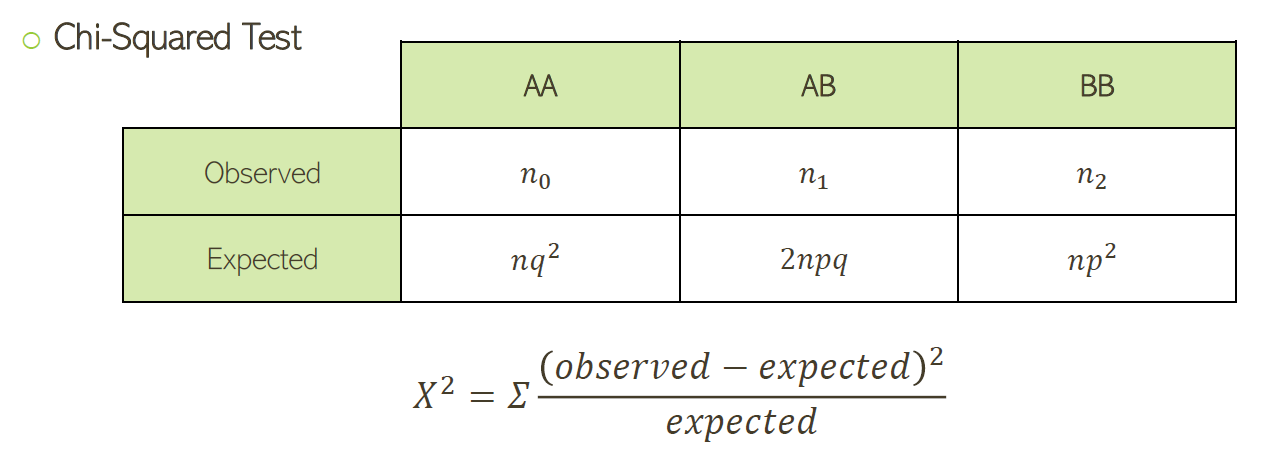
\includegraphics[width = \textwidth]{figs/chi-cuadrado.png}
\end{figure}

Mide lo que difiere los resultados observados con los resultados esperados. El problema es que con los GWAS, este test no es del todo preciso, por lo que se emplea el exact test.

Una vez calculado el HWE y con el test se ve cómo difieren los resultados, se ve si se está violando la ley de HW, es decir, si las frecuencias genotípicas son significativamente diferentes de las esperadas. En GWAS, se asume que desviaciones de HWE se deben a errores del genotipado. En el caso de estudios binarios, el límite del HWE es menos estricto en casos que en controles, ya que la violación de la ley puede indicar una asociación genética real con riesgo a enfermedad. Para estudios cuantitativos, se emplea un p-valor menor a 1e-6. 

\subsubsection{Heterocigosidad}
La heterocigosidad indica la proporción de loci heterocigotos en un individuo, es decir, se refiere a la presencia de los dos alelos en un SNP de un individuo. Se recomienda eliminar todos los individuos que se desvíen $\pm 3 SD$ de la media:
$$HeterozygosityRate_ind = \frac{NonMissingCounts - HomozygousGenotypeCount}{NonMissingCounts}$$
Un alto nivel de heterozigosidad se puede deber a una calidad baja de las muestras o contaminación, y unos niveles bajos a inbreeding o una relación entre las muestras.

\subsubsection{Relatedness}
Relatedness es el último paso del control de calidad. En los GWAS más comunes, se asume que no hay asociación entre los participantes del estudio. El grado de relatedness se puede definir como número de alelos compartidos entre los individuos dos a dos. Se mide mediante identity by descent (IBD), que es la proporción de los genomas de dos individuos compartiendo alelos heredados de un ancestro común. 

\begin{figure}[htbp]
\centering
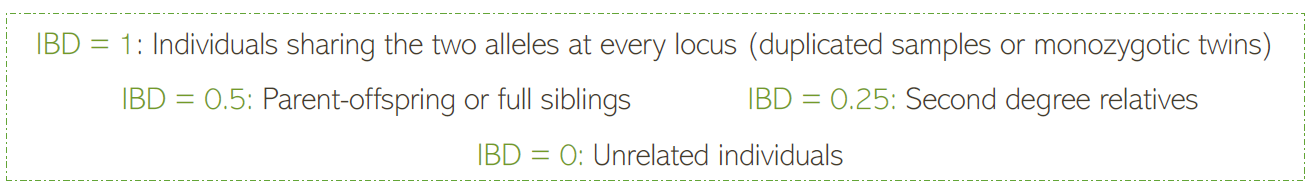
\includegraphics[width = \textwidth]{figs/ibd.png}
\end{figure}

Se diferencian Identity-by-state (IBS) de Identity-by-descent (IBD). En IBS, los alelos compartidos entre individuos son en un locus particular debido a evolución convergente, ancestros comunes o eventos mutacionales similares y se computa como sin información sobre herencia, mientras que en IBD los alelos compartidos entre individuos en un locus particular se debe a un ancestro comun y se debe estimar la probabilidad de heredad la misma copia de un alelo.

En estudios de población estándar, se recomienda eliminar uno de los individuos con un IBD mayor de 0,2. El desequilibrio de ligamiento hace referencia a la herencia conjunta de genes en diferentes loci en el mismo cromosoma en una población concreta. Los SNP están en LD cuando la frecuencia de asociación de sus alelos es superior a la esperada si los loci fueran independientes y estuvieran asociados al azar. 

\section{Práctica: Proyecto HapMap internacional}
El objetivo es elaborar un mapa de haplotipos del genoma humano. La información está disponible gratuitamente en conjuntos de datos públicos. Comenzó con una reunión, celebrada del 27 al 29 de octubre de 2002, y alcanzó su objetivo de completar el mapa en tres años. Se trata de una colaboración entre investigadores de centros académicos, grupos de investigación biomédica sin ánimo de lucro y empresas privadas de Japón, Reino Unido, Canadá, China, Nigeria y Estados Unidos. El HapMap identifica entre 250.000 y 500.000 SNP marcados (casi tanta información cartográfica como los 10 millones de SNP). Cuenta con muestras procedentes de Yoruba, Japón, China y Estados Unidos (residentes en Utah con ascendencia del norte y oeste de Europa).

Los haplotipos son un conjunto de alelos de un cromosomas que se han heredado conjuntamente de un mismo progenitor al estar localizados de forma próxima en el cromosoma. Se puede limitar a un solo gen o a múltiples. Los \textbf{TagSNP} son SNPs representativos en una región del genoma con un alto linkage disequilibrium. 

\begin{figure}[htbp]
\centering
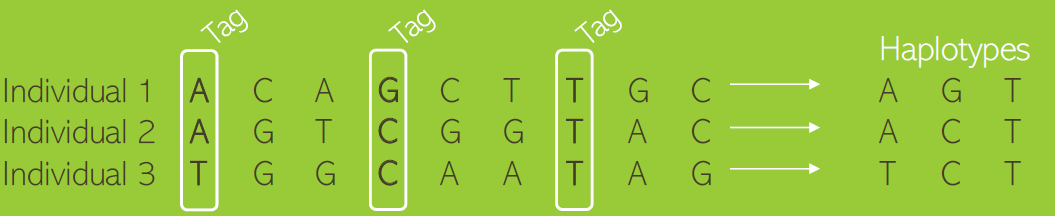
\includegraphics[width = \textwidth]{figs/tagsnp.png}
\end{figure}

El Proyecto Internacional HapMap nació para desarrollar un mapa de haplotipos del genoma humano. 

Durante las prácticas de esta parte de la asignatura, haremos uso de los datos del HapMap para determinar asociaciones entre los SNPs de este estudio y la variable de resultado, en lo que se conoce como estudios de asociación de genoma completo (GWAS).

Como ya hemos visto en clase, el control de calidad es el primer paso en los GWAS. Este proceso es crucial para eliminar las muestras de baja calidad, la contaminación, deshacerse de los errores generados durante el SNP calling o controlar la subestructura de la población, entre otras cosas. Esto es esencial para asegurar que nuestros datos tienen suficiente calidad para realizar las pruebas de asociación.

Como recordatorio, el control de calidad se divide en algunos pasos:
\begin{enumerate}
\item Control for missingness
\item Sex Discrepancy
\item Minor allele frequency
\item Hardy-Weinberg equilibrium
\item Heterozygosity
\item Relatedness
\item Population substructure
\end{enumerate}

En este pipeline, controlaremos los seis primeros pasos. Para ello se utilizará principalmente PLINK, una herramienta que permite estudiar las características de los datos y limpiarlos de forma sencilla y eficaz. También se utilizará R para trazar algunos resultados y ayudar en la determinación de los umbrales (librerías ggplot2 y dplyr).

\subsection{Missingness por individuo y por SNP}
La falta de datos (missingness) se refiere al grado de datos no disponibles a nivel de SNP o de individuo y está directamente asociada con la calidad de los datos. Una buena práctica consiste en eliminar los SNP/individuos con una elevada proporción de omisión.

Para determinar esta proporción, podemos utilizar `--missing` de PLINK. Este flag genera dos archivos que muestran la proporción de SNPs perdidos por individuo y la proporción de individuos perdidos por SNP, respectivamente. 

En este paso, se crean los ficheros plink.lmiss con la información de missigness de los SNP y plink.imiss con la información de missigness de los individuos.

\begin{lstlisting}[language=bash]
plink --bfile HapMap_3_r3_1 --missing --out plink
\end{lstlisting}

Como dice el informe, tenemos 1457897 variantes y 165 personas (80 hombres / 85 mujeres).

\subsection{Estudio de Missingness de SNP}

\begin{lstlisting}[language=R]
snpmiss <- read.table(file="plink.lmiss", header=TRUE)

kable(head(snpmiss), caption = "SNP missingness information") %>%
  kable_styling(bootstrap_options = c("striped", "hover", "condensed", "responsive"), full_width = FALSE) 
\end{lstlisting}

Una vez cargados los datos, los visualizamos:

\begin{lstlisting}[language=R]
p <- ggplot(snpmiss, aes(x=F_MISS)) +
  geom_histogram(color="black", fill="#E69F00", binwidth=.0025) +
  ggtitle('Histogram SNP missingness') +
  ylab('Frequency') +
  geom_vline(xintercept = .02, linetype="dotted",
               color = "black", linewidth=.9)
p 
\end{lstlisting}

\begin{figure}[htbp]
\centering
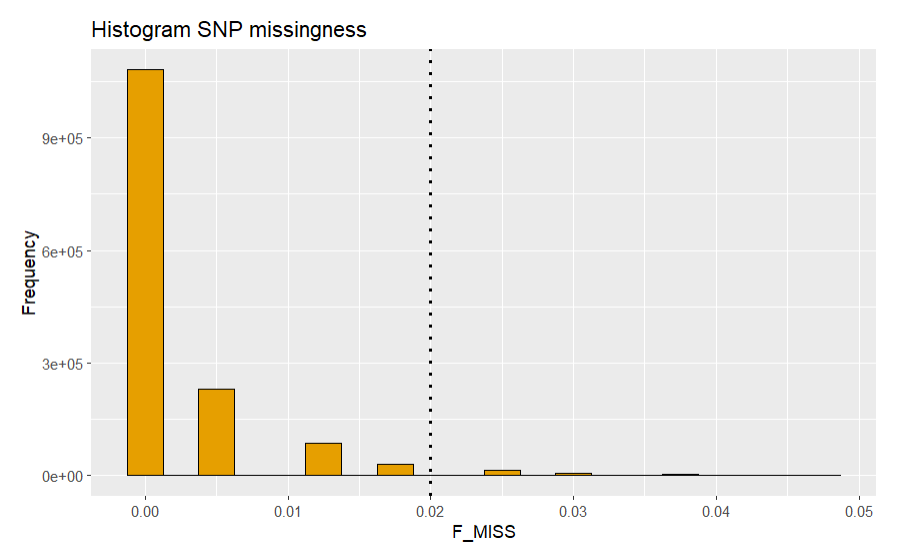
\includegraphics[width = 0.8\textwidth]{figs/hist-snpmiss.png}
\end{figure}

Imaginemos que decidimos fijar un umbral en 0,02. Esto significa que estamos eliminando SNPs con más del 2\% de su información faltante.
\begin{lstlisting}[language=R]
sum(snpmiss$F_MISS > 0.02)
\end{lstlisting}

En total estamos eliminando 27454 valores. Para ver la cantidad de individuos que deben tener una ausencia información para ese SNP para que se elimine, se realiza el siguiente código y el resultado son 4 personas.
\begin{lstlisting}[language=R]
deleted_snp <- snpmiss[snpmiss$F_MISS > 0.02, ]
min(deleted_snp$N_MISS)
\end{lstlisting}

\subsubsection{Estudio de missingness de individuos}
De forma similar a como hemos hecho con el SNP missingness, queremos detectar el missingness individual. Para ello, cargar el archivo que contiene esta información y, representar los individuos falta en un histograma:
\begin{lstlisting}[language=R]
indmiss <- read.table("plink.imiss", header = TRUE)

p <- ggplot(indmiss, aes(F_MISS)) +
  geom_histogram(color="black", fill="#E69F00", binwidth=.0005)

p
\end{lstlisting}

\begin{figure}[htbp]
\centering
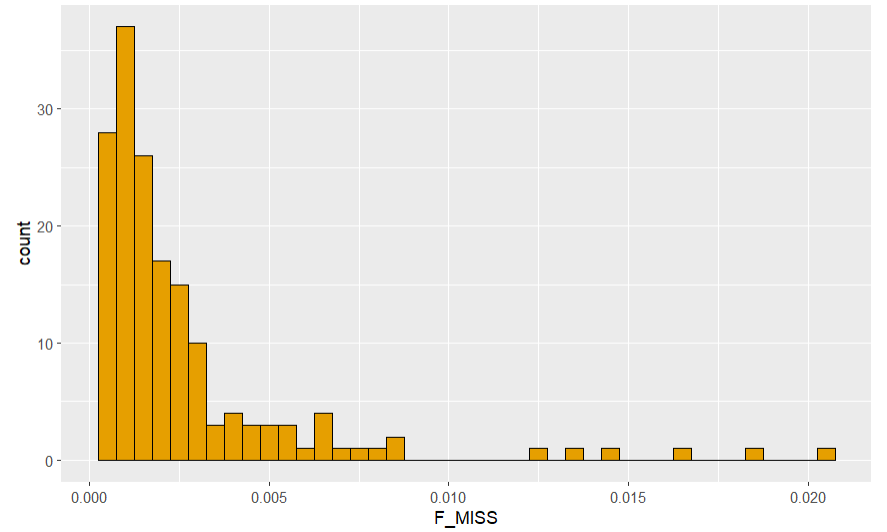
\includegraphics[width = 0.8\textwidth]{figs/hist-indmiss.png}
\end{figure}

Decidimos fijar de nuevo el umbral en 0,02. Esto significa que se eliminan los individuos con más de un 2\% de omisión en sus SNP, que en este caso es una persona.
\begin{lstlisting}[language=R]
sum(indmiss$F_MISS > 0.02)
\end{lstlisting}

Para ver la cantidad de SNPs que deben estar ausentes en un individuo para eliminarlo, se realiza el siguiente cálculo y el resultado son 29584.
\begin{lstlisting}[language=R]
deleted_ind <- indmiss[indmiss$F_MISS > 0.02, ]
min(deleted_ind$N_MISS)
\end{lstlisting}

\subsubsection{Filtrar SNPs e individuos}
Después de representar los resultados, concluimos que el 2\% de missingness es un buen umbral tanto para SNPs como para individuos. Por lo tanto, debemos utilizar `--geno` y `--mind` para eliminar ese porcentaje.

\begin{lstlisting}[language=bash]
# Delete SNPs with missingness >0.02.
plink --bfile HapMap_3_r3_1 --geno 0.02 --make-bed --out HapMap_3_r3_2

# Delete individuals with missingness >0.02.
plink --bfile HapMap_3_r3_2 --mind 0.02 --make-bed --out HapMap_3_r3_3
\end{lstlisting}

Tras analizar el output, vemos que no se ha eliminado ningún individuo. Esto se debe a que, como primero se eliminan los SNP, se recalcula el missingness para los individuos y el que antes sí eliminábamos, ya no cumple con la condición (los SNPs de los que no tenía información son aquellos que se han eliminado por tener poca información de individuos).

%02/12 - Lucía Sánchez
A continuación miramos la discrepancia entre sexos. La discrepancia de sexo se refiere a la diferencia entre el sexo asignado y el determinado. Puede estudiarse con `--check-sex`, que genera un documento con 6 columnas:
\begin{enumerate}
\item FID: family ID
\item IID: individual ID
\item PEDSEX: sex from the pedigree file (1 = male, 2 = female)
\item SNPSEX: sex determined by X chromosome
\item STATUS: problem/ok
\item F: the actual X chromosome inbreeding (homozygosity) estimate. This estimate allows to determine the sex of the individuals, being F < 0.2 assigned to females, and F > 0.8, to males.
\end{enumerate}

Primero utilizamos ese flag para determinar el número de personas con sexo masculino y femenino:
\begin{lstlisting}[language=bash]
plink --bfile HapMap_3_r3_3 --check-sex --out plink
\end{lstlisting}

Ese fichero se carga en R y se genera un histograma con F estimado:
\begin{lstlisting}[language=R]
sex <- read.table("plink.sexcheck", header = TRUE)
p <- ggplot(sex, aes(F)) +
  geom_histogram(color="black", fill="#E69F00", binwidth=.005)
p
\end{lstlisting}

Para ver el número de hombres y mujeres predichos:
\begin{lstlisting}[language=R]
#males
sum(sex$SNPSEX == 1)

#females
sum(sex$SNPSEX == 2)
\end{lstlisting}
Obtenemos 81 hombres y 84 mujeres. Ahora queremos ver si hay alguna discordancia entre el sexo predicho y el computado:
\begin{lstlisting}[language=R]
discordance <- sex[sex$PEDSEX != sex$SNPSEX,]
discordance
\end{lstlisting}

Vemos que hay un individuo que discrepa, por lo que queremos filtrarlo. Generamos un fichero .txt con el FID e IID de la persona problemática.
\begin{lstlisting}[language=bash]
grep "PROBLEM" plink.sexcheck | awk '{print $1, $2}' > sex_discrepancy.txt
\end{lstlisting}

Posteriormente utilizamos el flag --remove para eliminar los individuos en el fichero txt.
\begin{lstlisting}[language=bash]
plink --bfile HapMap_3_r3_3 --remove sex_discrepancy.txt --make-bed --out HapMap_3_r3_4
\end{lstlisting}

Ahora analizamos minor allele frequency (MAF). El MAF se refiere a la frecuencia del alelo menos frecuente en un locus. Debemos eliminar los SNP con un MAF bajo porque la potencia estadística de los GWAS no permite detectar asociaciones si la frecuencia del alelo es demasiado baja. Generamos un fichero .txt con los SNPs autosomales y después eliminamos aquellos con el MAF más pequeño. 
\begin{lstlisting}[language=bash]
# Select autosomal SNPs (from chromosomes 1 to 22).
awk '{ if ($1 >= 1 && $1 < 23) print $2}' HapMap_3_r3_4.bim > snp_1_22.txt
#Remove unlisted variants
plink --bfile HapMap_3_r3_4 --extract snp_1_22.txt --make-bed --out HapMap_3_r3_5
\end{lstlisting}

A continuación utilizamos el flag --freq para computar el MAF en los cromosomas autosomales.
\begin{lstlisting}[language=bash]
plink --bfile HapMap_3_r3_5 --freq --out plink
\end{lstlisting}

Cargamos el fichero generado y representamos la distribución de MAF en un histograma, estableciendo un límite del 5\%.
\begin{lstlisting}[language=R]
maf_freq <- read.table("plink.frq", header = TRUE)
p <- ggplot(maf_freq, aes(MAF)) +
	geom_histogram(color="black", fill="#E69F00", binwidth=.005) +
	geom_vline(xintercept = .05, linetype="dotted", color = "black", linewidth=.9)
p
\end{lstlisting}

Estamos eliminando 1073226 SNPs y quedándonos con 325318.
\begin{lstlisting}[language=R]
#deleting
sum(maf_freq$MAF >= 0.05)
#retaining
sum(maf_freq$MAF < 0.05)
\end{lstlisting}

Eliminamos los SNPs.
\begin{lstlisting}[language=bash]
plink --bfile HapMap_3_r3_5 --maf 0.05 --make-bed --out HapMap_3_r3_6
\end{lstlisting}

El siguiente paso es eliminar los SNPs que no estén en equilibrio Hardy-Weinberg. El equilibrio de Hardy-Weinberg (HWE) establece que, en un apareamiento aleatorio, las frecuencias alélicas y genotípicas permanecen constantes o estables en una población si no se introducen factores perturbadores. `--hardy` escribe una lista de recuentos de genotipos y estadísticas de la prueba exacta de equilibrio Hardy-Weinberg.
\begin{lstlisting}[language=bash]
plink --bfile HapMap_3_r3_6 --hardy --out plink
\end{lstlisting}

Posteriormente elegimos los SNPs con un p-valor HWE < 0,0001.
\begin{lstlisting}[language=bash]
awk '{ if ($9 <0.00001) print $0 }' plink.hwe > plinkzoomhwe.hwe
\end{lstlisting}

Y ahora creamos los histogramas:
\begin{lstlisting}[language=R]
hwe <- read.table("plink.hwe", header = TRUE)
hwe
p <- ggplot(hwe, aes(P)) +
  geom_histogram(color="black", fill="#E69F00", binwidth=.05)
p

hwe_zoom <- read.table("plinkzoomhwe.hwe", header = FALSE)
hwe_zoom
p <- ggplot(hwe_zoom, aes(V9)) +
  geom_histogram(color="black", fill="#E69F00")
p
\end{lstlisting}

\section{Consideraciones de GWAS}
En cuanto al diseño del estudio, pueden diferenciarse los estudios basados en población, en familia o en poblaciones aisladas.

\subsection{Population-based GWAS}
Se trata de un estudio de asociación genética con individuos no emparentados. El estudio más común es uno de casos y controles, siendo los casos personas con presencia de un fenotipo y los controles ausencia del mismo. Los individuos pueden seleccionarse activamente y los controles se pueden emparejar con los casos (con respecto al sexo, factores de riesgo, ...). Se realiza un reclutamiento activo. Estos estudios tienen buena potencia y son rentables si la frecuencia de la enfermedad en la población es baja (<20\%). Si la frecuencia de los casos es mayor que la frecuencia basada en población, se debe ajustar por covariantes durante el análisis estadístico. Los casos y controles que no se genotipen conjuntamente deben tener una corrección (batch correction) para ajustar por covariables.

Los estudios de casos y controles se pueden clasificar en estudios retrospectivos y prospectivos. En los \textbf{estudios retrospectivos}, los sujetos se seleccionan en función de su estado de enfermedad. Se suele utilizar con enfermedades raras, ya que no es viable escoger participantes y esperar a que generen la enfermedad. Se obtienen los datos genéticos y ambientales.

En los \textbf{estudios prospectivos}, se establece una cohorte y se realiza un genotipado base de todos los sujetos. Se realiza un seguimiento de los individuos y se observa si hay un desarrollo de la enfermedad. Aquellos que la desarrollen pasan a ser controles, y aquellos que no serán los controles. 

Las ventajas es que estos estudios son muy rentable para asociaciones a gran escala, pero tiene la desventaja de obtener subgrupos poblacionales, generando asociaciones falsas debido a las subpoblaciones.

\subsection{Family-based GWAS}
Este estudio utiliza sujetos recogidos en familias, y se utilizó frecuentemente en los inicios de GWAS. En el caso del trío caso-padres, se genotipa a la descendencia afectada y a los padres. Se compara entre el número de alelos marcadores transmitidos de padres a descendientes con el número de alelos no transmitidos. Se puede tralizar la prueba de desequilibrio de transmisión (TDT) o prueba de asociación para identificar el vínculo genético entre un marcador genético (SNP) y un rasgo (fenotipo). Examina la segregación de un alelo dentro de una familia. La ventaja es que es robusto frente a estratificación poblacional y con enfermedades de baja prevalencia (< 1\%). Además, se estudian los efectos de un alelo en un fenotipo individual de sus efectos indirectos en miembros familiares cercanos. No obstante, se requiere un tamaño muestral más grande que el GWAS poblacional para alcanzar la misma potencia estadística y es menos eficiente en el caso de enfermedades de aparición tardía.

\subsection{Poblaciones aisladas}
Las poblaciones aisladas son grupos separado de sus poblaciones vecinas por barreras (geográficas, culturales o lingüísticas) y que tienen un flujo genético mínimo desde ellas. Estas poblaciones aisladas han permanecido aisladas durante un periodo prolongado, teniendo un flujo genético restringido con las poblaciones vecinas. Estos estudios tienen una mayor precisión de imputación que otras pruebas con un desequilibrio de ligamiento de largo alcance. 
Los descubrimientos en poblaciones aisladas son muy difíciles de replicar en otras poblaciones. Así, variantes funcionales raras pueden estar presente en mayor frecuencia en poblaciones aisladas, habiendo así una potencia aumentada para estudios de asociación de estas variantes.

\subsection{Subestructura poblacional - práctica}
En esta práctica estudiaremos relatedness y la estratificación poblacional. La estratificación poblacional puede ser la principal fuente de confusión. Ejemplo: estudio de casos y controles, en el que las diferencias genotípicas entre casos y controles se deben a los distintos orígenes de la población (casos: europeos, controles: asiáticos) y no a un efecto sobre el riesgo de enfermedad. La confusión se debe a que la subestructura de la población no está distribuida por igual entre los grupos de casos y controles. Así, una señal de asociación surgirá no por una asociación entre un fenotipo y un SNP, sino por diferencias de frecuencia alélica entre las poblaciones que comprenden los casos y los controles. Esto tiene dos soluciones: eliminar los individuos de ascendencia divergente o establecer la ascendencia como covariable/efecto aleatorio en modelos mixtos.

Los métodos para identificación de individuos con diferencias a larga escala en ascendencia es mediante una PCA (principal component analysis) o MDS (multidimensional scaling). MDS calcula la proporción de alelos compartidos entre cada par de individuos para identificar la variación genética para cada individuo. Los resultados se muestran en un gráfico para explorar la distribución de individuos en los datos. Por ejemplo, estudio genético que incluya sujetos de Asia y Europa. El análisis MDS revelaría que los asiáticos son genéticamente más parecidos entre sí que a los europeos.

%04/12 - Lucía Sánchez
\chapter{Análisis estadístico o de asociación}
La imputación permite predecir otros SNPs no secuenciados debido a que se heredan conjuntamente, ampliando así la información de los SNPs. Los softwares que se pueden utilizar son:
\begin{itemize}
\item \textbf{IMPUTE2 y MACH}: utilizan un modelo de Markov oculto (HMM) para estimar los genotipos que faltan, mediante la inferencia de haplotipos y el uso de parámetros genéticos previamente especificados, como las tasas de mutación y de recombinación
\item \textbf{BEAGLE}: no necesita tales parámetros. Estima los valores que faltan mediante el uso de haplotipos agrupados localmente con algoritmos HMM y de maximización de expectativas (EM).
\end{itemize}

El test de asociación se realiza después de la imputación. El test de asociación que se realice depende del fenotipo (binario o continuo), el control de covariantes (edad, sexo) y la estructura poblacional (estratificación u homogeneidad), pudiendo ser regresiones lineales, regresiones lineales múltiples, modelos lineares mixtos, regresiones logísticas, etc. Los tipos de análisis que se pueden encontrar en función de la dominancia son:
\begin{itemize}
\item \textbf{Modelo dominante:} La presencia del alelo B aumenta el riesgo de enfermedad en la misma medida para los genotipos BB y AB, en comparación con el riesgo de referencia para los AA.
\item \textbf{Modelo codominante o aditivo:} Cada copia adicional del alelo B aumenta el riesgo de enfermedad de forma aditiva, o por el contrario, aumenta el efecto protector.
\item \textbf{Modelo recesivo:} Se necesitan dos copias del alelo B para expresar la característica fenotípica relacionada con este alelo.
\end{itemize}

\section{Tipos de test de asociación}
\subsection{Modelos lineares}
Se describen mediante la fórmula:
$$y = \beta_0 + \beta_1 \cdot X_{1i} + \epsilon_1$$

Siendo $y$ la variable dependiente (respuesta/outcome), $\beta_0$ el término constante del modelo, $\beta_1$ el coeficiente de regresión, $X_{1i}$ la variable independiente o predictora y $\epsilon_1$ el término del error. $i$ representa el número de observaciones o muestras.

Los cambios que se producen en el outcome (y) se puede modelar como una función lineal de la variable independiente. Así, un cambio en la variable independiente produce un cambio en la variable dependiente, siendo ésta numérica. 

Un ejemplo: Se desea estimar si el tabaco (medido como el número de cigarrillos fumados al mes) influye en el volumen residual pulmonar (VR: volumen de aire que queda en los pulmones tras una espiración máxima). Si existe una asociación entre el tabaco y el VR, el número de cigarrillos (variable independiente) se asociaría con una reducción del VR (variable dependiente)

En este caso, la variable predictora va a ser categórica, representando los distintos SNPs. Normalmente, el estimador (la pendiente) suele estar relacionado con el p-valor. 

\subsection{Modelos de regresión lineal múltiple}
Se incluyen otros predictores o covariables. Los términos en la variable dependiente se modelan con todos los predictores independientes. Una manera de regular la estratificación de la población es metiéndolo como covariable.

Siguiendo con el ejemplo previo, nos damos cuenta de que el volumen residual puede verse afectado no sólo por el número de cigarrillos fumados al mes, sino también por la edad y el sexo. Ahora tendremos tres variables independientes para probar la dependiente: tabaco, sexo y edad.

\subsection{Modelos lineares mixtos}
Estos modelos sirven para modelar estructuras de datos más complejas. Las variables predictoras se dividen en dos:
\begin{itemize}
\item \textbf{Efecto fijo:} son las variable que se espera que tengan un efecto en la variable respuesta. Un ejemplo sería los SNP y el entorno o las covariables clínicas.
\item \textbf{Efectos aleatorios:} no nos interesa su impacto en la variable de respuesta, pero sabemos que pueden estar influyendo en los patrones que observamos, por lo que queremos separarlos del modelo para ver cómo verdaderamente el efecto fijo afecta al outcome. Aquí se contarían variables categóricas que queremos controlar.
\end{itemize}

Un ejemplo sería un estudio de la deprivación del sueño. Se restringe el tiempo de sueño de 18 individuos y la reacción de su organismo durante 10 días. El objetivo es determinar cómo cambia la reacción de los individuso durante su deprivación de sueño. Si se mide como regresión lineal simple, la variabilidad va cambiando. Si se clusteriza cada dato por individuo, se puede ver que la recta que se traza es más ajustada a los datos, demostrando que hay una estructura compleja que no se puede determinar por un modelo lineal.

\begin{table}[htbp]
\centering
\begin{tabular}{p{7cm}|p{7cm}}
Modelo de regresión lineal & Modelos mixtos \\ \hline
Suponen una relación lineal entre las variables dependientes e independientes. & Relajan el supuesto de independencia entre las observaciones. \\
\\
Adecuado para analizar datos con una estructura simple (se supone que las observaciones son independientes entre sí). & Adecuado para analizar datos con una estructura agrupada (las observaciones están anidadas dentro de grupos / mediciones repetidas en los mismos sujetos). \\
\\
Los modelos de regresión lineal suelen incluir efectos fijos: parámetros asociados a las variables predictoras. Estos efectos son constantes en todos los niveles de cualquier variable de agrupación. & Los modelos mixtos incluyen efectos fijos (como los modelos lineales) y efectos aleatorios (captan la variabilidad a distintos niveles).\\
\\
Tareas de regresión simple: se desea predecir una variable de resultado continua a partir de una o más variables predictoras. & Se utilizan en análisis de datos longitudinales, análisis de medidas repetidas y modelización jerárquica. Son apropiados cuando los datos no son independientes y se desea tener en cuenta las correlaciones dentro del grupo o la variabilidad específica de los sujetos.
\end{tabular}
\end{table}

\subsection{Regresión logística}
La regresión logística sigue la fórmula:
$$y = \frac{e^{(\beta_0 + \beta_1X_{1i)}}}{1 + e^{(\beta_0 + \beta_1X{1i})}}$$

Los cambios en la variable dependiente (y) pueden modelizarse como una función logística de las variables independientes. Hay dos variantes:
El modelo de regresión logística múltiple es como la lineal múltiple, pero logística, es decir, se añaden varias variables independientes. El modelo multinomial cuenta con una variable dependiente con más de dos categorías.

Siguiendo con el ejemplo, nos interesa detectar si existe una asociación entre el número de cigarrillos: (variable independiente continua) y el volumen residual inferior a 1 litro (variable dependiente binaria: sí/no). En la regresión logística múltiple, se añadiría sexo como covariable, mientras que en la regresión logística multinomial la variable dependiente tendría más de dos categorías.

\section{Visualización de datos}
El plot se denomina como Manhattan plot. Las asociaciones significativas se muestran en la parte superior del gráfico. El eje x va por orden en los distintos cromosomas. 

\begin{figure}[htbp]
\centering
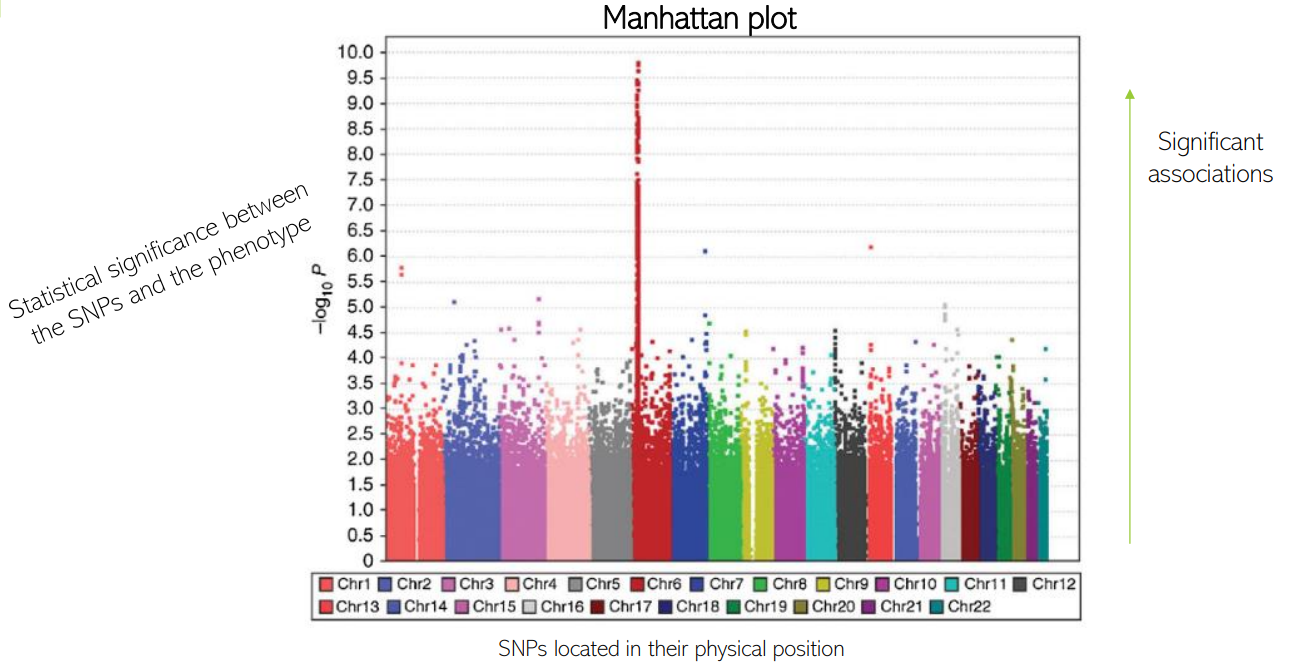
\includegraphics[width = \textwidth]{figs/manhattan-plot.png}
\end{figure}

\section{Nivel de significancia de GWAS}
A la hora de mirar el nivel de significancia de GWAS, nos encontramos con el problema del testeo múltiple. El p-valor representa la probabilidad de obtener resultados tan extremos como los observados si la hipótesis nula es correcta. La hipótesis nula dice que no hay una relación significativa entre el predictor y la variable respuesta. El nivel de significancia se suele poner en 0,05. 

Por ejemplo, estamos probando (hipótesis nula) que no hay una relación significativa entre el predictor (SNP, edad y sexo) con la variable respuesta (volumen residual). Si el p-valor es 0,03, si no hubiera una relación entre esas variables (y la hipótesis nula fuera cierta), la probabilidad de tener resultados tan extremos como los observados sería de 0,03. 

Con un nivel de significancia de 0,05, todavía hay una probabilidad de que no haya una relación significativa, aunque sea pequeña. Esto no es un problema cuando se realiza un solo análisis, pero cuando se realizan muchos, se incrementa el número de falsos positivos. Por ello, se debe controlar el testo múltiple y ajustar el p-valor. Esto se puede realizar de varias formas:
\begin{itemize}
\item \textbf{Corrección de Bonferroni:} divide el nivel de significancia por el número de análisis realizados para ver el nivel de significancia que se debe comprobar en cada análisis individual. No obstante, es algo restrictivo, incrementando los falsos negativos.
\item \textbf{False Discovery Rate (FDR):} se describió por Benjamini y Hochberg en 1995, y monitoriza el número de falsos positivos en relación al número de resultados positivos, siendo así menos estricto.
\end{itemize}